\documentclass{article}

% Required packages
\usepackage{amssymb}
\usepackage{amsmath}
\usepackage{graphicx}
\usepackage{geometry}
\usepackage{tikz}
\usepackage{array}
\usepackage{booktabs}
\usepackage{enumitem}
\usepackage{listings}
\usepackage{xcolor}
\usepackage{fancyhdr}
\usepackage{float}
\usepackage{subcaption}
\usepackage{comment}

% Set page geometry
\geometry{a4paper, margin=1in}

% Configure listings for Python
\lstset{
  language=Python,
  basicstyle=\ttfamily\footnotesize,
  numbers=left,
  numberstyle=\tiny\color{gray},
  frame=single,
  breaklines=true,
  breakatwhitespace=true,
  captionpos=b,
  tabsize=4,
  showspaces=false,
  showstringspaces=false,
  showtabs=false,
  commentstyle=\color{gray}\textit,
  keywordstyle=\color{blue}\bfseries,
  stringstyle=\color{red}
}

\begin{document}

\pagestyle{fancy}
\chead{DSC 257: Unsupervised Learning (Fall 2025)}
\lhead{Homework 2}
\rhead{Randall Rogers}

%------------------
% Solution for 1(a) 
%------------------
\subsection*{Solution 1}
\noindent\rule{\textwidth}{0.4pt}\\

\subsubsection*{Solution 1 (a)}
\subsubsection*{Define $\ell_1$}
\parbox{\textwidth}{
$\ell_1$ or $||x||_1$ is defined as:
$$\ell_{1} = ||x||_1 = \sum_{i=1}^{d} |x_{i}| $$
}
\subsubsection*{Compute $\ell_1$}
\parbox{\textwidth}{
Let $x=\begin{bmatrix} 1 \\ -2 \\ 3 \end{bmatrix}$ \\

\begin{align*}
  ||x||_1 &= \sum_{i=1}^{3} |x_{i}| \\
  &= |x_{1}| + |x_{2}| + |x_{3}| \\
  &= |1| + |-2| + |3| \\
  &= 1 + 2 + 3 \\
  &= 6
\end{align*}
}


\subsubsection*{\normalfont}{$\therefore$ $||x||_{1} = 6$}

\noindent\rule{\textwidth}{0.4pt}\\

\newpage

%------------------
% Solution for 1(b) 
%------------------
\subsection*{Solution 1}
\noindent\rule{\textwidth}{0.4pt}\\

\subsubsection*{Solution 1 (b)}
\subsubsection*{Define $\ell_2$}
\parbox{\textwidth}{
$\ell_2$ or $||x||_2$ is defined as:
$$\ell_{2} = ||x||_2 = \sqrt{\sum_{i=1}^{d} x_{i}^2} $$
}
\subsubsection*{Compute $\ell_2$}
\parbox{\textwidth}{
Let $x=\begin{bmatrix} 1 \\ -2 \\ 3 \end{bmatrix}$ \\

\begin{align*}
  ||x||_2 &= \sqrt{\sum_{i=1}^{3} x_{i}^{2}} \\
  &= \sqrt{x_{1}^2 + x_{2}^{2} + x_{3}^{2}} \\
  &= \sqrt{1^{2} + (-2)^{2} + 3^{2}} \\
  &= \sqrt{1 + 4 + 9} \\
  &= \sqrt{14}
\end{align*}
}


\subsubsection*{\normalfont}{$\therefore$ $||x||_{2} = \sqrt{14}$}

\noindent\rule{\textwidth}{0.4pt}\\

\newpage

%------------------
% Solution for 1(c) 
%------------------
\subsection*{Solution 1}
\noindent\rule{\textwidth}{0.4pt}\\

\subsubsection*{Solution 1 (c)}
\subsubsection*{Define $\ell_{\infty}$}
\parbox{\textwidth}{
$\ell_{\infty}$ or $||x||_{\infty}$ is defined as:
$$\ell_{\infty} = ||x||_{\infty} = \text{max}_{i}\left|x_{i}\right| $$
}
\subsubsection*{Compute $\ell_{\infty}$}
\parbox{\textwidth}{
Let $x=\begin{bmatrix} 1 \\ -2 \\ 3 \end{bmatrix}$ \\

\begin{align*}
  ||x||_{\infty} &= \text{max}(\{|x_{1}|,|x_{2}|,|x_{3}|\}) \\
  &= \text{max}(\{|1|,|-2|,|3|\}) \\
  &= \text{max}(\{1,2,3\}) \\
  &= 3 \\
\end{align*}
}


\subsubsection*{\normalfont}{$\therefore$ $||x||_{\infty} = 3$}

\noindent\rule{\textwidth}{0.4pt}\\

\newpage


%------------------
% Solution for 1(b)
%------------------
\subsection*{Solution 1}
\noindent\rule{\textwidth}{0.4pt}\\

\subsubsection*{Solution 1 (b)}
\subsubsection*{Define $\ell_2$}
\parbox{\textwidth}{
$\ell_2$ or $||x||_2$ is defined as:
$$\ell_{2} = ||x||_2 = \sqrt{\sum_{i=1}^{d} x_{i}^{2} }$$
}


\subsubsection*{\normalfont}{$\therefore$ we can express the dataspace $\chi$ as: $\chi = \mathbb{R}^{10}$}

\noindent\rule{\textwidth}{0.4pt}\\

\subsubsection*{Solution 1 (b)}
\subsubsection*{Step 1: Identify characteristics of the dataspace}
\parbox{\textwidth}{
We are given 3 dimensional vectors where each element is zero or one ($x_{i} \in [0,1]$):
}

\subsubsection*{\normalfont}{$\therefore$ we can express the dataspace $\chi$ as: $\chi = {[0,1]}^{3}$}

\noindent\rule{\textwidth}{0.4pt}\\

\newpage

%------------------
% Solution for 2(a),2(b), and 2(c)
%------------------
\subsection*{Solution 2}
\noindent\rule{\textwidth}{0.4pt}\\
\subsubsection*{Solution 2 (a)}
\subsubsection*{Step 1: Define Euclidean distance ($\ell_2$)}
\parbox{\textwidth}{

$$\ell_2 = \|p - q\|_2 = \sqrt{\sum_{i=1}^{n} (p_i - q_i)^2}$$

}

\subsubsection*{Step 2: Compute $\ell_2$}
\parbox{\textwidth}{
Let $p=1$ and $q=10$
$$
\begin{aligned}
\ell_2 &= \sqrt{\sum_{i=1}^{n} (p_i - q_i)^2}\\
\ell_2 &= \sqrt{\sum_{i=1}^{1} (1 - 10)^2}\\
\ell_2 &= \sqrt{(- 9)^2}\\
\ell_2 &= 9
\end{aligned}
$$
}
\subsubsection*{\normalfont}{$\therefore$ $\ell_{2} = 9$}

\noindent\rule{\textwidth}{0.4pt}\\

\subsubsection*{Solution 2 (b)}
\subsubsection*{Step 1: Define Euclidean distance ($\ell_2$)}
\parbox{\textwidth}{

$$\ell_2 = \|p - q\|_2 = \sqrt{\sum_{i=1}^{n} (p_i - q_i)^2}$$

}

\subsubsection*{Step 2: Compute $\ell_2$}
\parbox{\textwidth}{
Let $p = \begin{bmatrix} -1 \\ 12 \end{bmatrix}, q = \begin{bmatrix} 6 \\ -12 \end{bmatrix}$
$$
\begin{aligned}
\ell_2 &= \sqrt{\sum_{i=1}^{n} (p_i - q_i)^2}\\
\ell_2 &= \sqrt{(p_1 - q_1)^{2}+(p_2 - q_2)^{2}}\\
\ell_2 &= \sqrt{(-1 - 6)^{2}+(12 - (-12))^{2}}\\
\ell_2 &= \sqrt{(-7)^{2}+(24)^{2}}\\
\ell_2 &= \sqrt{625}\\
\ell_2 &= 25
\end{aligned}
$$
}
\subsubsection*{\normalfont}{$\therefore$ $\ell_{2} = 25$}

\noindent\rule{\textwidth}{0.4pt}\\


\subsection*{Solution 2}
\noindent\rule{\textwidth}{0.4pt}\\
\subsubsection*{Solution 2 (c)}
\subsubsection*{Step 1: Define Euclidean distance ($\ell_2$)}
\parbox{\textwidth}{

$$\ell_2 = \|p - q\|_2 = \sqrt{\sum_{i=1}^{n} (p_i - q_i)^2}$$

}

\subsubsection*{Step 2: Compute $\ell_2$}
\parbox{\textwidth}{
Let $p = \begin{bmatrix} 1 \\ 5 \\ -1 \end{bmatrix}, q = \begin{bmatrix} 5 \\ 2 \\ 11 \end{bmatrix}$
$$
\begin{aligned}
\ell_2 &= \sqrt{\sum_{i=1}^{n} (p_i - q_i)^2}\\
\ell_2 &= \sqrt{(p_1 - q_1)^{2}+(p_2 - q_2)^{2}+(p_3 - q_3)^{2}}\\
\ell_2 &= \sqrt{(1 - 5)^{2}+(5 - 2)^{2}+(-1 - 11)^{2}}\\
\ell_2 &= \sqrt{(-4)^{2}+(3)^{2}+(-12)^{2}}\\
\ell_2 &= \sqrt{169}\\
\ell_2 &= 13
\end{aligned}
$$
}
\subsubsection*{\normalfont}{$\therefore$ $\ell_{2} = 13$}

\noindent\rule{\textwidth}{0.4pt}\\

\newpage

%------------------
% Solution for 3(a) and 3(b)
%------------------
\subsection*{Solution 3}
\noindent\rule{\textwidth}{0.4pt}\\
\subsubsection*{Solution 3 (a)}
\subsubsection*{Step 1: Normalize the vector $x$}
\parbox{\textwidth}{
Let $x = \begin{bmatrix} 10 \\ 15 \\ 25 \end{bmatrix}$

$$\sum_{i=1}^{3} x_{i} = x_{1} + x_{2} + x_{3} = 10 + 15 + 25 = 50$$

Now, divide each entry by the total sum:\\

$$p = \frac{1}{50} \cdot x = \frac{1}{50} \begin{bmatrix} 10 \\ 15 \\ 25 \end{bmatrix} = \begin{bmatrix} 10/50 \\ 15/50 \\ 25/50 \end{bmatrix} = \begin{bmatrix} 0.2 \\ 0.3 \\ 0.5 \end{bmatrix}$$
}
\subsubsection*{\normalfont}{$\therefore$ the result ($p$) of scaling vertor $x$ is the following:}
$$p = \begin{bmatrix} 0.2 \\ 0.3 \\ 0.5 \end{bmatrix}$$ \\

\noindent\rule{\textwidth}{0.4pt}\\

\subsubsection*{Solution 3 (b)}
\subsubsection*{Step 1: Define dimension of the probability simplex}
\parbox{\textwidth}{
The dimension of vector $p$ is $3$ and $k=n-1$ where $k$ is the dimension of the probability simplex
}
\subsubsection*{\normalfont}{$\therefore$ vector $p$ lies in the probability simplex($\Delta_2$) for $k=2$}

\noindent\rule{\textwidth}{0.4pt}\\

\newpage

%------------------
% Solution for 4
%------------------
\subsection*{Solution 4}
\noindent\rule{\textwidth}{0.4pt}\\

\subsubsection*{Step 1: Define probability simplex $\Delta_2$ }
\parbox{\textwidth}{

For a point to be scalable to $\Delta_2$, after scaling it must satisfy:
\begin{itemize}
\item All components must be non-negative
\item The sum of components must equal 1
\end{itemize}
}

\subsubsection*{Step 2: Give example that violates one of the rules in Step 1}
\parbox{\textwidth}{
Let $x = \begin{bmatrix} 1 \\ -2 \end{bmatrix}$

The second component of $x$ violates the first rule, all components for a point must be non-negative $\Delta_2$.
}

\subsubsection*{\normalfont}{$\therefore$ the point $x = \begin{bmatrix} 1 \\ -2 \end{bmatrix}$ cannot be scaled to lie in $\Delta_{2}$}

\noindent\rule{\textwidth}{0.4pt}\\

\newpage

%------------------
% Solution for 5
%------------------
\subsection*{Solution 5}
\noindent\rule{\textwidth}{0.4pt}\\

\subsubsection*{Visualizing the Simplex $\Delta_3$ in 2D Projections}
\parbox{\textwidth}{
Here are the three 2D views of the probability simplex $\Delta_3$. Each plot is a \textit{shadow} of the 3D triangle, viewed along one of the principal axes.
}

%---------------------------------------------------
%  FIGURE 1: x1 vs x2 Projection
%---------------------------------------------------
\begin{figure}[h!]
\centering
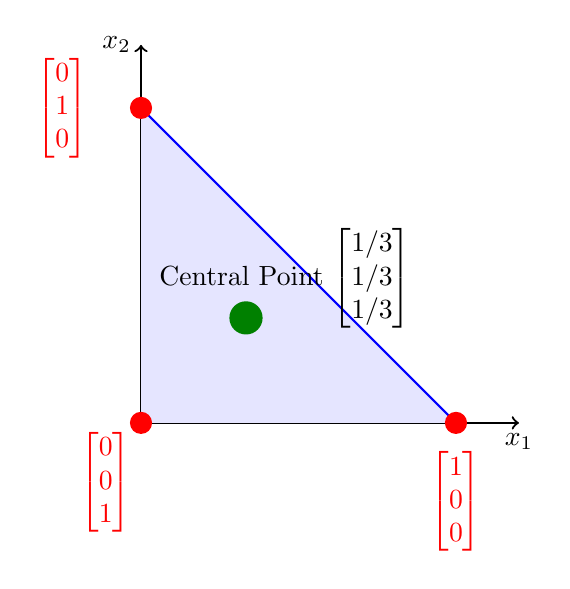
\begin{tikzpicture}[scale=4]
    % Axes
    \draw[->, thick] (0,0) -- (1.2,0) node[below] {$x_1$};
    \draw[->, thick] (0,0) -- (0,1.2) node[left] {$x_2$};

    % The projected simplex region (x1 + x2 <= 1)
    \fill[blue!10] (0,0) -- (1,0) -- (0,1) -- cycle;
    \draw[blue, thick] (1,0) -- (0,1);

    % The three vertices of the simplex
    \fill[red] (1,0) circle (1pt) node[shift={(0, -1)}] {$\begin{bmatrix} 1 \\ 0 \\ 0 \end{bmatrix}$};
    \fill[red] (0,1) circle (1pt) node[shift={(-1, 0)}] {$\begin{bmatrix} 0 \\ 1 \\ 0 \end{bmatrix}$};
    \fill[red] (0,0) circle (1pt) node[below left] {$\begin{bmatrix} 0 \\ 0 \\ 1 \end{bmatrix}$};

    % The central point (centroid)
    \fill[green!50!black] (1/3, 1/3) circle (1.5pt) node[shift={(0.5,0.5)}, black] {Central Point $\begin{bmatrix} 1/3 \\ 1/3 \\ 1/3 \end{bmatrix}$};
\end{tikzpicture}
\caption{View 1: Projection onto the $x_1$-$x_2$ plane.}
\label{fig:x1x2}
\end{figure}

%---------------------------------------------------
%  FIGURE 2: x2 vs x3 Projection
%---------------------------------------------------
\begin{figure}[h!]
\centering
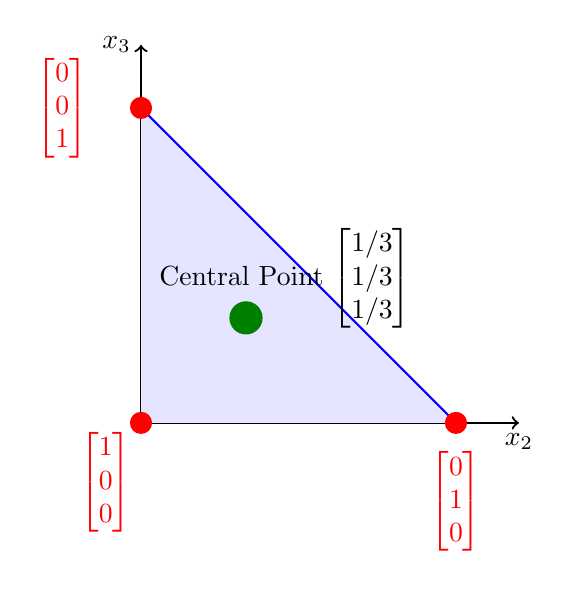
\begin{tikzpicture}[scale=4]
    % Axes
    \draw[->, thick] (0,0) -- (1.2,0) node[below] {$x_2$};
    \draw[->, thick] (0,0) -- (0,1.2) node[left] {$x_3$};

    % The projected simplex region (x2 + x3 <= 1)
    \fill[blue!10] (0,0) -- (1,0) -- (0,1) -- cycle;
    \draw[blue, thick] (1,0) -- (0,1);

    % The three vertices of the simplex
    \fill[red] (1,0) circle (1pt) node[shift={(0, -1)}] {$\begin{bmatrix} 0 \\ 1 \\ 0 \end{bmatrix}$};
    \fill[red] (0,1) circle (1pt) node[shift={(-1, 0)}] {$\begin{bmatrix} 0 \\ 0 \\ 1 \end{bmatrix}$};
    \fill[red] (0,0) circle (1pt) node[below left] {$\begin{bmatrix} 1 \\ 0 \\ 0 \end{bmatrix}$};

    % The central point (centroid)
    \fill[green!50!black] (1/3, 1/3) circle (1.5pt) node[shift={(0.5,0.5)}, black] {Central Point $\begin{bmatrix} 1/3 \\ 1/3 \\ 1/3 \end{bmatrix}$};
\end{tikzpicture}
\caption{View 2: Projection onto the $x_2$-$x_3$ plane.}
\label{fig:x2x3}
\end{figure}

\newpage

\subsection*{Solution 5}
\noindent\rule{\textwidth}{0.4pt}\\
%---------------------------------------------------
%  FIGURE 3: x1 vs x3 Projection
%---------------------------------------------------
\begin{figure}[h!]
\centering
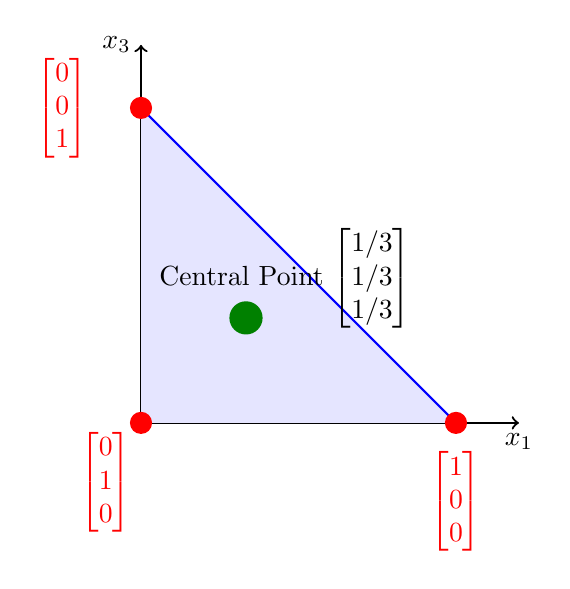
\begin{tikzpicture}[scale=4]
    % Axes
    \draw[->, thick] (0,0) -- (1.2,0) node[below] {$x_1$};
    \draw[->, thick] (0,0) -- (0,1.2) node[left] {$x_3$};

    % The projected simplex region (x1 + x3 <= 1)
    \fill[blue!10] (0,0) -- (1,0) -- (0,1) -- cycle;
    \draw[blue, thick] (1,0) -- (0,1);

    % The three vertices of the simplex
    \fill[red] (1,0) circle (1pt) node[shift={(0, -1)}] {$\begin{bmatrix} 1 \\ 0 \\ 0 \end{bmatrix}$};
    \fill[red] (0,1) circle (1pt) node[shift={(-1, 0)}] {$\begin{bmatrix} 0 \\ 0 \\ 1 \end{bmatrix}$};
    \fill[red] (0,0) circle (1pt) node[below left] {$\begin{bmatrix} 0 \\ 1 \\ 0 \end{bmatrix}$};

    % The central point (centroid)
    \fill[green!50!black] (1/3, 1/3) circle (1.5pt) node[shift={(0.5,0.5)}, black] {Central Point $\begin{bmatrix} 1/3 \\ 1/3 \\ 1/3 \end{bmatrix}$};
\end{tikzpicture}
\caption{View 3: Projection onto the $x_1$-$x_3$ plane.}
\label{fig:x1x3}
\end{figure}

\noindent\rule{\textwidth}{0.4pt}\\

\newpage

%------------------
% Solution for 6
%------------------
\subsection*{Solution 6}
\noindent\rule{\textwidth}{0.4pt}\\

\subsubsection*{6 (a): $\ell_1$ for $p$ and $q$}

\parbox{\textwidth}{The $\ell_1$ distance between two vectors $p, q \in \mathbb{R}^n$ is given by:
$$\|p-q\|_1 = \sum_{i=1}^n |p_i - q_i|$$

Let $p = \begin{bmatrix} 1/2 \\ 1/4 \\ 1/8 \\ 1/8 \end{bmatrix}$ and $q = \begin{bmatrix} 1/4 \\ 1/4 \\ 1/4 \\ 1/4 \end{bmatrix}$

\begin{align*}
    \|p-q\|_1 &= \left|\frac{1}{2} - \frac{1}{4}\right| + \left|\frac{1}{4} - \frac{1}{4}\right| + \left|\frac{1}{8} - \frac{1}{4}\right| + \left|\frac{1}{8} - \frac{1}{4}\right| \\
    &= \left|\frac{2}{4} - \frac{1}{4}\right| + |0| + \left|\frac{1}{8} - \frac{2}{8}\right| + \left|\frac{1}{8} - \frac{2}{8}\right| \\
    &= \frac{1}{4} + 0 + \left|-\frac{1}{8}\right| + \left|-\frac{1}{8}\right| \\
    &= \frac{1}{4} + \frac{1}{8} + \frac{1}{8} = \frac{2}{8} + \frac{1}{8} + \frac{1}{8} = \frac{4}{8} = \frac{1}{2}
\end{align*}
}
\subsubsection*{\normalfont}{$\therefore$ $\ell_{1}= \frac{1}{2}$}

\noindent\rule{\textwidth}{0.4pt}\\

\newpage

\subsection*{Solution 6}
\noindent\rule{\textwidth}{0.4pt}\\

\subsubsection*{6 (b): $\ell_1$ for $q$ and $r$}
\parbox{\textwidth}{The $\ell_1$ distance between two vectors $q, r \in \mathbb{R}^n$ is given by:
$$\|q-r\|_1 = \sum_{i=1}^n |q_i - r_i|$$

Let $q = \begin{bmatrix} 1/4 \\ 1/4 \\ 1/4 \\ 1/4 \end{bmatrix}$ and $r = \begin{bmatrix} 1/2 \\ 0 \\ 1/4 \\ 1/4 \end{bmatrix}$

\begin{align*}
\|q-r\|_1 &= \sum_{i=1}^{4} |q_i - r_i| \\
&= \left|\frac{1}{4} - \frac{1}{2}\right| + \left|\frac{1}{4} - 0\right| + \left|\frac{1}{4} - \frac{1}{4}\right| + \left|\frac{1}{4} - \frac{1}{4}\right| \\
&= \left|\frac{1}{4} - \frac{2}{4}\right| + \left|\frac{1}{4}\right| + |0| + |0| \\
&= \left|-\frac{1}{4}\right| + \frac{1}{4} + 0 + 0 \\
&= \frac{1}{4} + \frac{1}{4} \\
&= \frac{1}{2}
\end{align*}
}

\subsubsection*{\normalfont}{$\therefore$ $\ell_1 = \frac{1}{2}$}

\noindent\rule{\textwidth}{0.4pt}\\

\newpage

\subsection*{Solution 6}
\noindent\rule{\textwidth}{0.4pt}\\

\subsubsection*{6 (c): KL divergence $K(p, q)$}
\parbox{\textwidth}{
The Kullback-Leibler (KL) divergence from a distribution $p$ to a distribution $q$ is defined as:
$$K(p, q) = \sum_{i} p_i \ln \frac{p_i}{q_i}$$
Let $p = \begin{bmatrix} 1/2 \\ 1/4 \\ 1/8 \\ 1/8 \end{bmatrix}$ and $q = \begin{bmatrix} 1/4 \\ 1/4 \\ 1/4 \\ 1/4 \end{bmatrix}$
}

\begin{align*}
K(p, q) &= \sum_{i=1}^{4} p_i \ln\left(\frac{p_i}{q_i}\right) \\
&= p_1 \ln\left(\frac{p_1}{q_1}\right) + p_2 \ln\left(\frac{p_2}{q_2}\right) + p_3 \ln\left(\frac{p_3}{q_3}\right) + p_4 \ln\left(\frac{p_4}{q_4}\right) \\
&= \frac{1}{2}\ln\left(\frac{1/2}{1/4}\right) + \frac{1}{4}\ln\left(\frac{1/4}{1/4}\right) + \frac{1}{8}\ln\left(\frac{1/8}{1/4}\right) + \frac{1}{8}\ln\left(\frac{1/8}{1/4}\right) \\
&= \frac{1}{2}\ln(2) + \frac{1}{4}\ln(1) + \frac{1}{8}\ln\left(\frac{1}{2}\right) + \frac{1}{8}\ln\left(\frac{1}{2}\right) \\
&= \frac{1}{2}\ln(2) + \frac{1}{4}(0) - \frac{1}{8}\ln(2) - \frac{1}{8}\ln(2) \\
&= \frac{1}{2}\ln(2) - \frac{2}{8}\ln(2) \\
&= \left(\frac{1}{2} - \frac{1}{4}\right)\ln(2) \\
&= \frac{1}{4}\ln(2)
\end{align*}

\subsubsection*{\normalfont{$\therefore$ $K(p,q) = \frac{1}{4}\ln(2)$}}
\noindent\rule{\textwidth}{0.4pt}\\

\newpage

\subsection*{Solution 6}
\noindent\rule{\textwidth}{0.4pt}\\

\subsubsection*{6 (d): KL divergence $K(q, r)$}
\parbox{\textwidth}{
The Kullback-Leibler (KL) divergence from a distribution $q$ to a distribution $r$ is defined as:
$$K(q, r) = \sum_{i} q_i \ln \frac{q_i}{r_i}$$
Let $q = \begin{bmatrix} 1/4 \\ 1/4 \\ 1/4 \\ 1/4 \end{bmatrix}$ and $r = \begin{bmatrix} 1/2 \\ 0 \\ 1/4 \\ 1/4 \end{bmatrix}$ \\

Looking at the second component ($i=2$). Here, $q_2 = \frac{1}{4} > 0$ while $r_2 = 0$. The corresponding term in the KL divergence sum, $q_2 \ln\left(\frac{q_2}{r_2}\right)$, involves division by zero. \\

Hence, the divergence will be infinite.
}
\subsubsection*{\normalfont}{$\therefore$ $K(q, r) = \infty$}

\noindent\rule{\textwidth}{0.4pt}\\

\newpage

\end{document}